\chapter{РЕАЛИЗАЦИЯ ГЕНЕРАТОРА ШИМ}
\section{Постановка задачи}	
Требуется разработать модель цифрового логического устройства объёме ПЛИС Spartan-3E XC3S500E4PQ208C, сочетающую в себе
функциональные узлы делителя частоты 1кГц, фильтра дребезга контактов
кнопки и конечного автомата генератора последовательности.

Центральным узлом схемы является 64-разрядный сдвиговый регистр.
Исходное состояние сдвигового регистра определяется заданной в виде вектор-функции таблицей истинности (см. Таблицу~\ref{tab:4func-vector}).


\begin{table}[h!]
	\centering
	\small
	\caption{Вектор-функция}
	\begin{tabular}{|c|c|c|c|c|c|c|c|c|c|c|c|c|c|c|c|}
		\hline
		F & E & D & C & B & A & 9 & 8 & 7 & 6 & 5 & 4 & 3 & 2 & 1 & 0 \\ \hline\hline
		0 & 4 & 4 & 8 & 3 & 0 & 7 & 2 & 2 & D & 7 & C & 5 & 2 & A & C \\ \hline
	\end{tabular}
	\label{tab:5func-vector}
\end{table}

Сдвиговый регистр после снятия сигнала асинхронного сброса RST
должен содержать значения, соответствующие варианту, как показано на
Рисунке~\ref{fig:set-reset}.


\begin{figure}
	\centering
	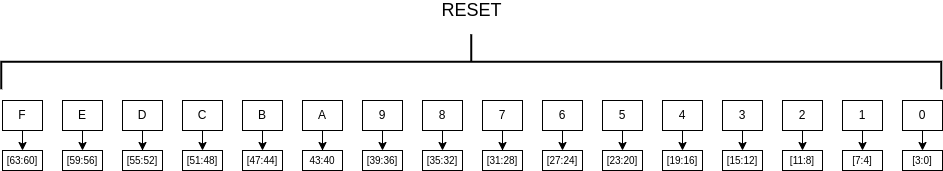
\includegraphics[width=0.75\linewidth]{course-plis/images/lab5/set-reset}
	\caption{Исходное состояние сдвигового регистра}
	\label{fig:set-reset}
\end{figure}



Во время штатного функционирования, при деактивированном сигнале
сброса RST сдвиговый регистр способен выполнять две операции.
Первая операция --- циклический сдвиг влево на 4 разряда, выполняется при
<<1>> на входе SHIFT\_4B\_L, как показано на Рисунке~\ref{fig:leftshift}.

\begin{figure}[h!]
	\centering
	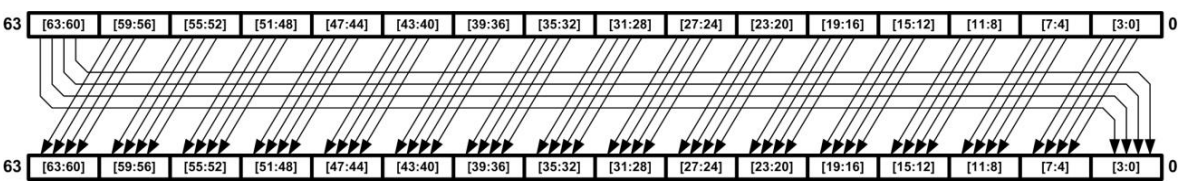
\includegraphics[width=0.8\linewidth]{course-plis/images/lab4/left_shift}
	\caption{Операция сдвига влево}
	\label{fig:leftshift}
\end{figure}

Вторая операция – циклический сдвиг вправо на 4 разряда, выполняется
при <<0>> на входе SHIFT\_4B\_L и <<1>> на входе SHIFT\_4B\_R, как показано на Рисунке~\ref{fig:rightshift}.


\begin{figure}[h!]
	\centering
	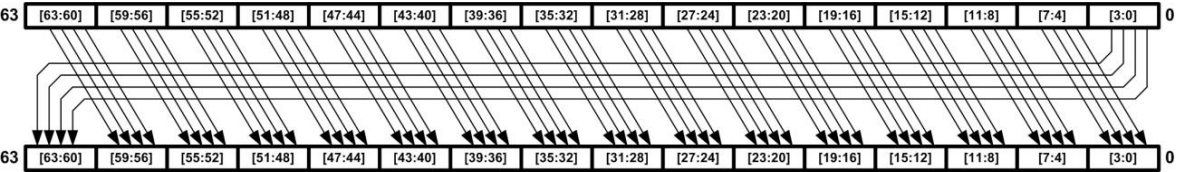
\includegraphics[width=0.8\linewidth]{course-plis/images/lab4/right_shift}
	\caption{Операция сдвига вправо}
	\label{fig:rightshift}
\end{figure}





Сигналы, управляющие сдвиговым регистром, формируются фильтрами
дребезга контактов по нажатию на две пользовательские кнопки.
Выходы сдвигового регистра подаются на два блока индикации.

Первый блок использует светодиоды общего назначения, которые
управляются в режиме регулировки яркости свечения с помощью широтноимпульсного сигнала.

Второй блок индикации использует матричный индикатор, на который
выводятся все 64 разряда сдвигового регистра. Блок управления матричным индикатором коммутирует разряды сдвигового регистра согласно Рисунку~\ref{fig:display-out}.
Такая организация вывода позволяет увидеть изображение, выводимое на
индикатор, непосредственно на временной диаграмме.


\begin{figure}[h!]
	\centering
	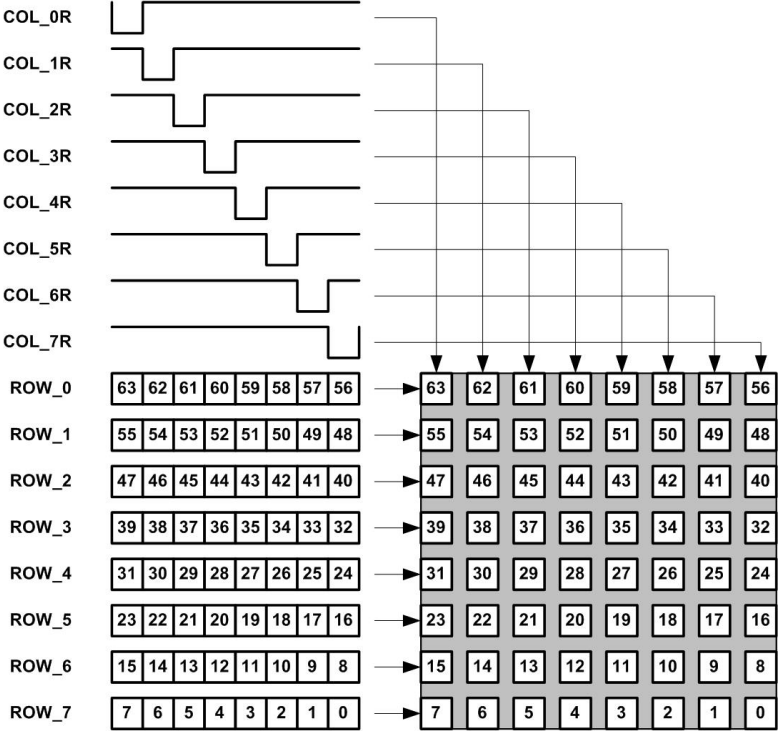
\includegraphics[width=0.45\linewidth]{course-plis/images/lab4/display-out}
	\caption{Вывод содержимого регистра на матричный индикатор}
	\label{fig:display-out}
\end{figure}


В процессе выполнения задания необходимо описать на
языке Verilog модель генератора широтно-импульсного сигнала, имеющий интерфейс, приведенный на Рисунке~\ref{fig:pwm-interface}.

\begin{figure}[h!]
	\centering
	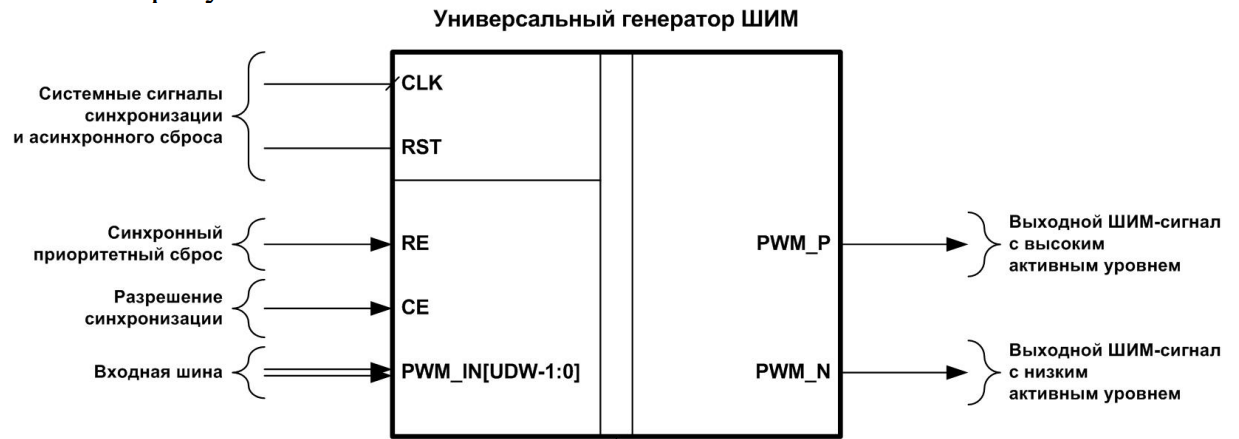
\includegraphics[width=0.55\linewidth]{course-plis/images/lab4/pwm-interface}
	\caption{Интерфейс генератора широтно-импульсного сигнала}
	\label{fig:pwm-interface}
\end{figure}


\section{Принцип широтно-импульсной модуляции}
Принцип широтно-импульсной модуляции (Pulse-Width
Modulation --- \\PWM) заключается в использовании двух уровней сигнала:
низкого и высокого, или <<0>> и <<1>>, соответственно, чередующихся с
фиксированным периодом, но с различной длительностью каждого уровня в
объёме периода.


\section{Реализация генератора ШИМ}


Синтезируемая модель генератора ШИМ-сигналов имеет параметр UDW,
определяющий разрядность входной шины и число состояний управляющего
автомата в объёме периода сигнала (частоту дискретизации). 

Именно этот
параметр обеспечивает универсальность модели.

\begin{figure}[h!]
	\centering
	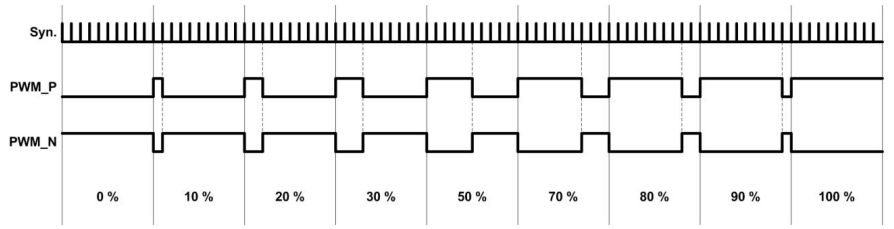
\includegraphics[width=0.6\linewidth]{course-plis/images/lab4/5principe}
	\caption{Принцип широтно-импульсной модуляции}
	\label{fig:5principe}
\end{figure}


%\begin{table}[h!]
%	\centering
%	\small
%	\begin{tabular}{|c|p{0.6\linewidth}|}
%		\hline
%		Параметр & Назначение \\ \hline
%		UDW & Определяет разрядность входной шины и число состояний управляющего
%		автомата в объёме периода сигнала (частоту дискретизации) \\ \hline
%		PWM\_P & Выходной ШИМ-сигнал с высоким активным сигналом \\\hline
%		PWM\_N & Выходной ШИМ-сигнал с низким активным сигналом \\\hline
%	\end{tabular}
%\end{table}
Число возможных входных комбинаций PWM\_IN, задающих коэффициент
заполнения периода активным уровнем сигнала (<<1>> -- для PWM\_P, <<0>> -- для
PWM\_N), составляет $2UDW$ штук. При этом комбинация из всех <<0>> задаёт
коэффициент 0\%, а комбинация из всех <<1>> – коэффициент 100\%. 

Период выходного сигнала делится на ($2UDW-1$) равных тактов, заданных частотой
сигнала разрешения синхронизации CE, либо равных периоду синхросигнала
CLK, если на вход CE подана константа <<1>>. Таким образом, частота
выходного ШИМ-сигнала получается из частоты дискретизации (частоты CE
или CLK при CE = <<1>>) путём деления на коэффициент ($2UDW-1$).



Граф переходов конечного автомата показан на Рисунке~\ref{fig:5graph}.
Состояние входного регистра изменяется в последнем такте
предпоследнего состояния автомата $(2UDW - 2)$.

\begin{figure}[h!]
	\centering
	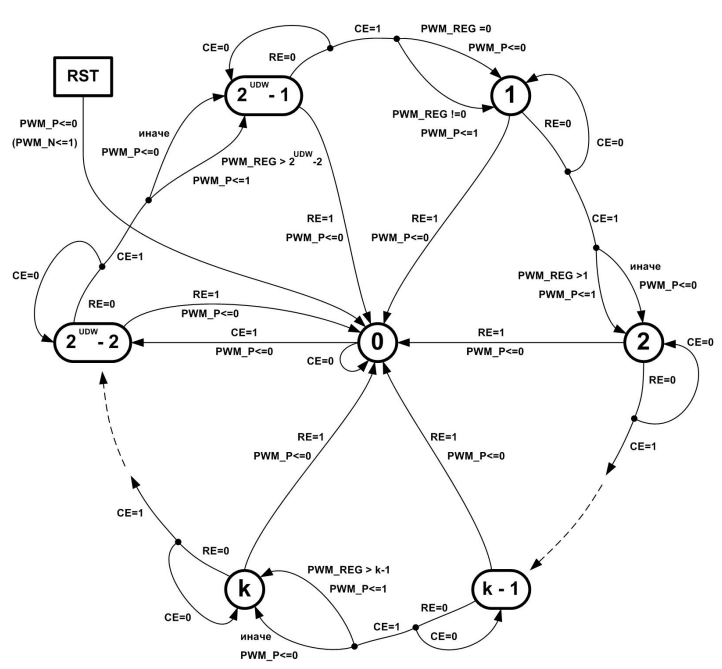
\includegraphics[width=0.55\linewidth]{course-plis/images/lab4/graph}
	\caption{Граф переходов конечного автомата}
	\label{fig:5graph}
\end{figure}

Входной регистр позволяет закончить период генерации ШИМ-сигнала на
основе неизменной управляющей комбинации, зафиксированной перед
началом текущего периода. 

Период генерации начинается в состоянии $2UDW - 1$ и заканчивается в состоянии $2UDW - 2$. Таким образом, изменения
комбинации на входе PWM\_IN не приведут к искажению формы выходного
сигнала.

Вход синхронного сброса RE предназначен для возврата автомата в
исходное состояние --- 0 и для перевода выходов в пассивное состояние.
Синхронный сброс является приоритетной операцией и воздействует
независимо от разрешения синхронизации CE. 

На входной регистр
PWM\_REG синхронный сброс не оказывает воздействия.
Временная диаграмма начала цикла работы генератора после синхронного
сброса показана на Рисунке~\ref{fig:sync-rst}. 

\begin{figure}[h!]
	\centering
	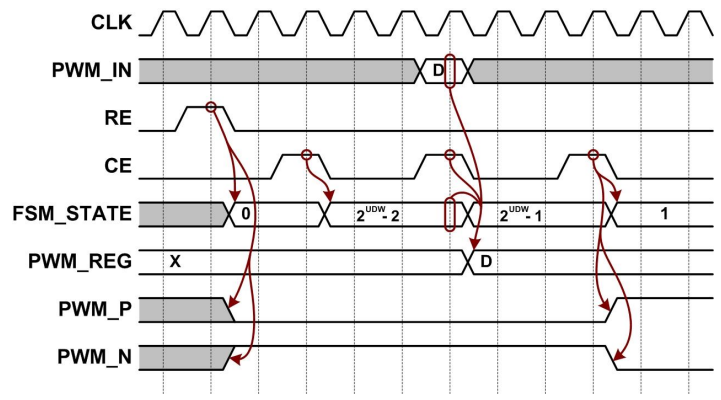
\includegraphics[width=0.54\linewidth]{course-plis/images/lab4/sync-rst}
	\caption{Синхронный сброс генератора}
	\label{fig:sync-rst}
\end{figure}




\section{Создание проекта САПР Xilinx ISE}
Приступим к реализации модели цифрового узла. Функциональная схема генератора ШИМ-сигналов приведена на
Рисунке~\ref{fig:func-scheme}.

\begin{figure}[h!]
	\centering
	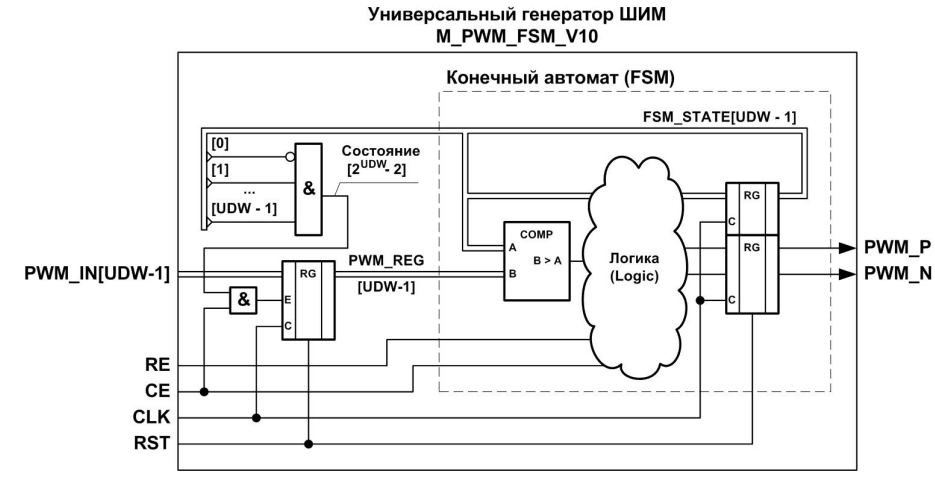
\includegraphics[width=0.65\linewidth]{course-plis/images/lab4/func-scheme}
	\caption{Функциональная схема генератора}
	\label{fig:func-scheme}
\end{figure}

Перечислим функциональные узлы, которые уже были реализованы ранее. 

\begin{enumerate}
	\item Делитель частоты. Реализован в разделе~\ref{cha:lab2}.
	\item Фильтр дребезга кнопок. Реализован в разделе~\ref{cha:lab2}.
	\item Конечный автомат генератор последовательности. Реализован в разделе~\ref{cha:lab2}.
	\item Блок управления матричным индикатором. Реализован в разделе~\ref{cha:lab4}.
\end{enumerate}

\paragraph{ШИМ генератор.}
Опишем на языке программирования Verilog модуль, реализующий ШИМ генератор. 
Исходный код данного функционального блока приведен в Приложении~\ref{cha:appendix1} в Листинге~\ref{lst:5pwm}.


\paragraph{Сдвиговый регистр.}
Опишем на языке программирования Verilog 64-разрядный сдвиговый регистр. Данный модуль реализует две операции:
\begin{enumerate}
	\item Циклический сдвиг влево на 4 разряда.
	\item Циклический сдвиг вправо на 4 разряда
\end{enumerate}

Исходный код данного функционального блока приведен в Приложении~\ref{cha:appendix1} в Листинге~\ref{lst:5shift}.

\paragraph{Блок управления матричным индикатором.}
Изменим модуль, реализующий блок управления матричным индикатором --- установим новый способ отображения входных сигналов на дисплей согласно Рисунку~\ref{fig:display-out}.

\begin{lstlisting}[caption={Измененный способ коммутации}]
	always@*
	begin
		rows = {data[63-column_ctr],
				data[55-column_ctr],
				data[47-column_ctr],
				data[39-column_ctr],
				data[31-column_ctr],
				data[23-column_ctr],
				data[15-column_ctr],
				data[7-column_ctr]
				};
	end
\end{lstlisting}

Исходный код данного функционального блока приведен в Приложении~\ref{cha:appendix1} в Листинге~\ref{lst:5lcd}.

\paragraph{Модуль верхнего уровня.}
Реализуем на языке Verilog модуль верхнего уровня.
Исходный код данного модуля приведен в Приложении~\ref{cha:appendix1} на Листинге~\ref{lst:5top}.

\paragraph{Тестовый модуль.}
Приступим к реализации модуля, который будет организовывать тестовое окружение рассматриваемой части цифрового логического устройства. В модуле верхнего уровня опишем генератор тактового сигнала частотой 48 МГц. Который будет использован в качестве тактового сигнала для всех синхронных функциональных узлов в составе устройства. 

Сигнал с частотой 1МГц будет использоваться как сигнал разрешения счета для генераторов ШИМ-сигналов, счетчика столбцов.

Исходный код данного модуля приведен в Приложении~\ref{cha:appendix1} в Листинге~\ref{lst:5test-top}.





\section{Тестирование и отладка средствами симулятора ISim}
После компоновки проекта, подключения модуля верхнего уровня, проведем верификацию спроектированных моделей с помощью симулятора iSim из состава САПР Xilinx ISE Design Suite. Результаты тестирования можно видеть в Приложении~\ref{cha:appendix2} на Рисунках~\ref{fig:5isim1}.~\ref{fig:5isim2}.





\section{Вывод}

В данном разделе нами были получены общие навыки работы с программным обеспечением Xilinx ISE Design Suite, изучены основы языка Verilog.

С помощью полученных знаний был спроектирован функциональный узел--генератор ШИМ сигналов, который был использован для управления светодиодными индикаторами, а также 64-рязрядный сдвиговый регистр.


